% Preamble

\documentclass{article}

% Packages

\usepackage{graphicx}
\usepackage[export]{adjustbox}

\usepackage{xcolor, colortbl}
\usepackage{booktabs}
\usepackage{arydshln}

\usepackage[T1]{fontenc}

%\usepackage{minted}
\usepackage{listings}
\lstset{
	%language=VHDL,
	basicstyle=\footnotesize\ttfamily}
%\usepackage[margin=0.5in]{geometry}

\usepackage[labelsep=period,  labelfont=bf]{caption}
%\usepackage[table,x11names]{xcolor}
%format=plain

\newcommand{\includecode}[2][c]{\lstinputlisting[]{#2}}


\begin{document}
	\pagenumbering{gobble}
	\addtolength{\topmargin}{-.5in} %.85, 55
	%\addtolength{\topmargin}{-3in} %.85, 55
	\begin{figure}%[ht]
	\includecode{example.mif}
	\captionsetup{width=1.55\textwidth, labelfont=bf,singlelinecheck=true, justification=justified}
	\caption{Machine code stored in source file $EXAMPLE.MIF$, created using the Simple Computer assembler. These instructions are executed on the $SCOMP$ and are used to compute $A = (B+C) + D$.}
	\end{figure}
	\vspace{3pt}
	%\inputminted{vhdl}{SM_VHDL.VHD}
	\begin{figure}%[hb]
		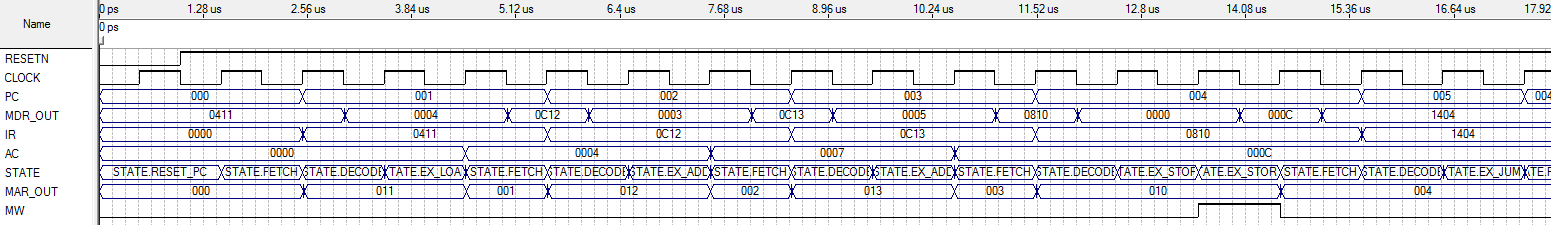
\includegraphics[scale=0.5,center]{waveform.PNG} %.43
		\captionsetup{width=1.55\textwidth, labelfont=bf,singlelinecheck=true, justification=justified}
		\caption{Timing simulation waveform of instructions stored in $EXAMPLE.MIF$ being executed on $SCOMP$. A 1 us period is used, and $RESETN$ is initially held $LOW$ to reset the computer. Once the reset signal is pulled $HIGH$, a $FETCH$ and $DECODE$ cycle is performed to load the next instruction, $EX\_LOAD$.}
		%\end{figure}
	\end{figure}
	\vspace{3pt}
	\begin{figure}%[hb]
		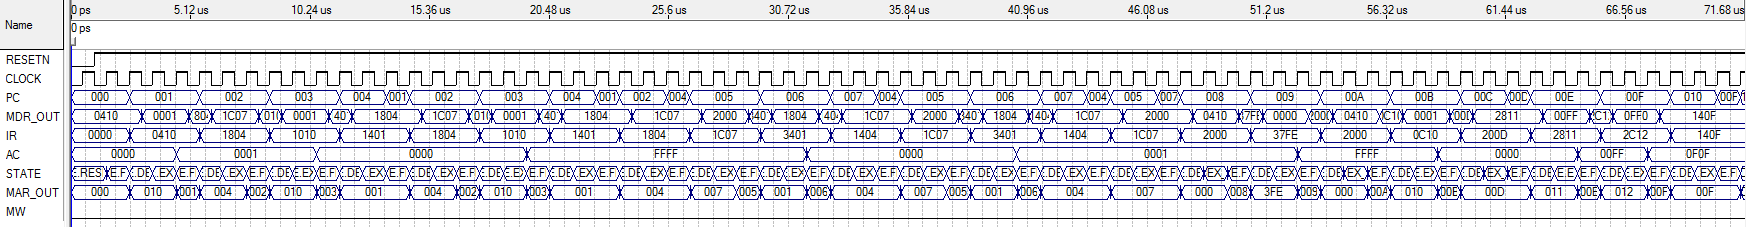
\includegraphics[scale=0.45,center]{sim_comp.PNG}
		\captionsetup{width=1.55\textwidth, labelfont=bf,singlelinecheck=true, justification=justified}
		%\caption{Waveform of state machine inputs $X[1:0]$, $CLOCK$, and $RESETN$ undergoing changes in time. Outputs $Q[1:0]$ and $Z$ will be given values once the simulation is run.}
		\caption{Timing simulation waveform of $SCOMP$, now with an extended number of instruction states, executing instructions stored in $TEST\_CODE.MIF$. The clock frequency is set to 1 us, and the $RESETN$ line is initially held $LOW$ to reset the computer. The $AC$ register ultimately retains the value 0x0F0F.}
	\end{figure}
	\vspace{3pt}
	\begin{figure}%[ht]
		\vspace{48pt}
		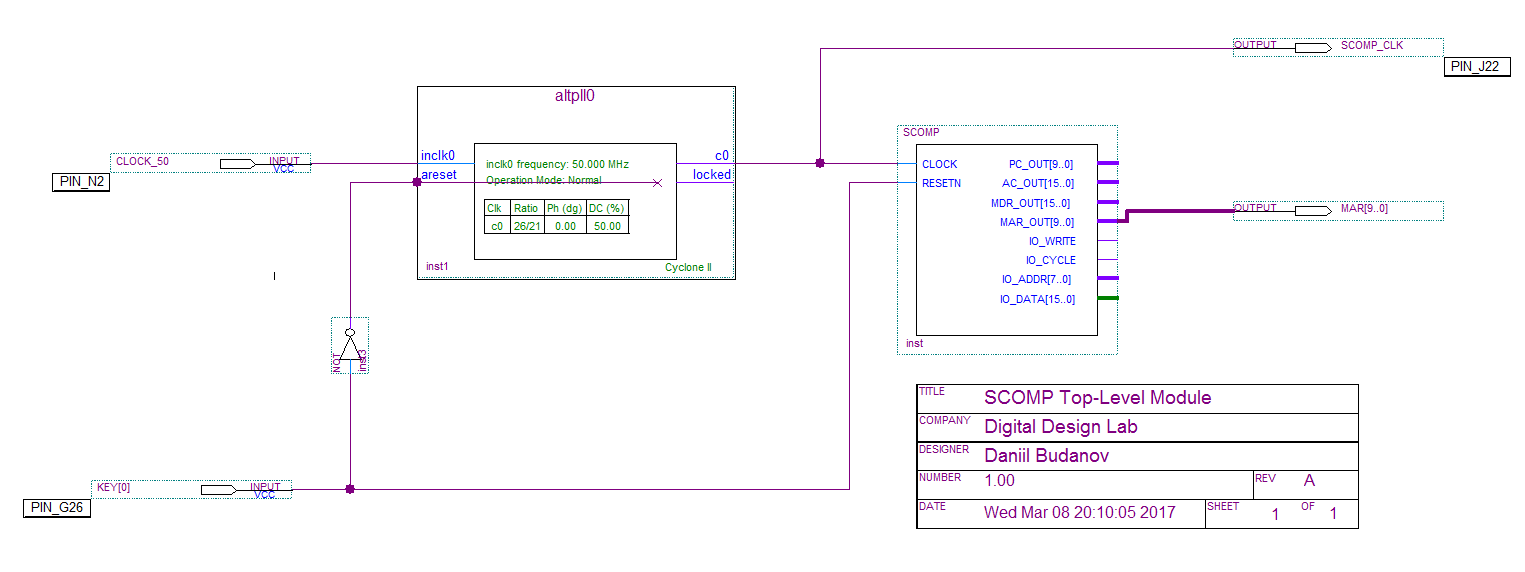
\includegraphics[scale=0.5,center]{schematic.PNG} %.549, .513
		\captionsetup{width=1.55\textwidth, labelfont=bf,singlelinecheck=true, justification=justified}
		%\caption{Functional simulation of a state machine with clock $CLOCK$, flip-flop resets $RESETN$, inputs $X[1:0]$ and outputs $Q[1:0]$ and $Z$.}
		\caption{Schematic of Simple Computer with a PLL being input a 50 MHz clock from the $DE2$ board and supplying a clock signal at 61.90 MHZ. This clock output frequency is within 5 MHz of the 65.03 MHz operating maximum of $SCOMP$, as given by the Timing Summary. $KEY[0]$ is used to reset both the PLL and the $SCOMP$, and the PLL output is routed to a physical pin $J22$ on the FPGA.}
		%\hline
	\end{figure}
		\vspace{3pt}
	\begin{figure}[ht]%[ht]
		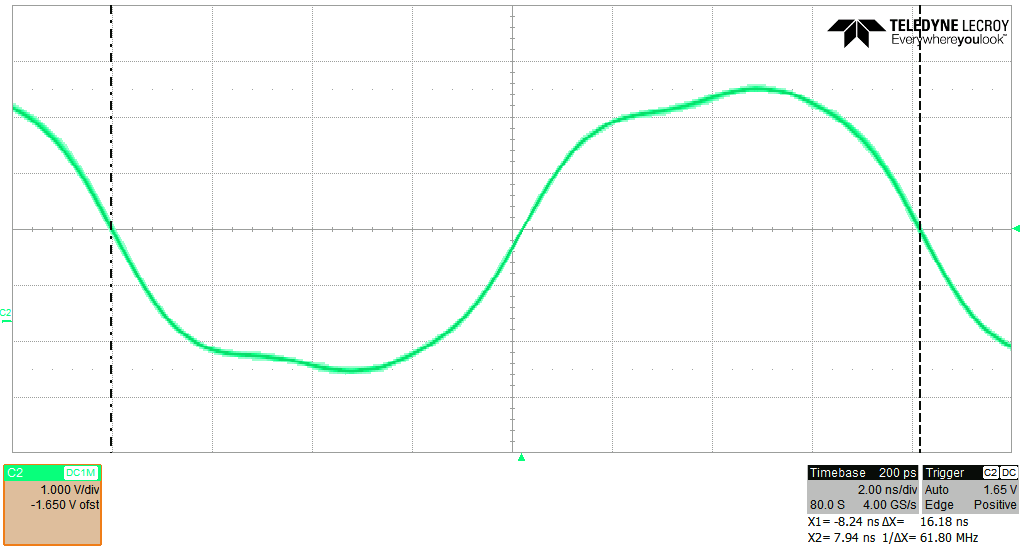
\includegraphics[scale=0.5,center]{clock_freq.png} %.549, .513
		\captionsetup{width=1.55\textwidth, labelfont=bf,singlelinecheck=true, justification=justified}
		%\caption{Functional simulation of a state machine with clock $CLOCK$, flip-flop resets $RESETN$, inputs $X[1:0]$ and outputs $Q[1:0]$ and $Z$.}
		\caption{Oscilloscope waveform of the clock signal being output by the PLL into the $SCOMP$. A 16.18 ns clock period is measured.}
		%\hline
	\end{figure}
\end{document}